\documentclass[11pt,a4paper]{article}
\usepackage[T1]{fontenc}
\usepackage[utf8]{inputenc}
\usepackage{amsmath,amsthm,newtxtext,newtxmath}
\usepackage[margin=23mm,headheight=14pt,headsep=7mm,footskip=11mm]{geometry}
\usepackage{microtype,graphicx,booktabs,tabularx,array,fancyhdr,xcolor,enumitem}
\usepackage{caption,tikz,float}
\usetikzlibrary{arrows.meta,positioning}
\usepackage[colorlinks=true,allcolors=blue!45!black,breaklinks=true]{hyperref}
\definecolor{ink}{HTML}{193944}\definecolor{teal}{HTML}{137C82}
\pagestyle{fancy}\fancyhf{}
\fancyhead[L]{\small\sffamily Pandrosion geometry and analog root computation}
\fancyhead[R]{\small\sffamily V30 / Research preprint}
\fancyfoot[C]{\small\thepage}\renewcommand{\headrulewidth}{.3pt}
\setlength{\parindent}{0pt}\setlength{\parskip}{5pt plus 1pt}
\setlength{\emergencystretch}{3em}\renewcommand{\arraystretch}{1.15}
\captionsetup{font=small,labelfont=bf}
\setlist{noitemsep,topsep=3pt,leftmargin=*}
\newtheorem{proposition}{Proposition}
\newcommand{\repo}{\url{https://github.com/ivan-fr/pandrosion}}
\hypersetup{pdftitle={Pandrosion Geometry and Analog Root Computation: Centered Binary Powers and a Precision--Time Study},pdfauthor={Ivan Besevic}}
\begin{document}
\thispagestyle{empty}
{\small\sffamily\color{teal} GEOMETRY / FORMAL ARITHMETIC / MIXED-SIGNAL SIMULATION}\par
\vspace{8pt}
{\fontsize{24}{27}\selectfont\bfseries\color{ink} Pandrosion Geometry and\\Analog Root Computation\par}
\vspace{6pt}
{\large Centered binary powers and a precision--time study}\par
\vspace{9pt}
Ivan Besevic\quad$\cdot$\quad Independent research\par
{\small Version 30\quad$\cdot$\quad19 September 2026}
\vspace{8pt}\hrule\vspace{8pt}
\textbf{Abstract.}
We translate a proportional-rectangle realization of classical Halley iteration into a programmable behavioral analog root calculator. Digital interval preparation supplies a scale $c$ and a normalized input $Y\approx Xc^p\in[1,2]$. The analog state $q=p(u-1)$ and centered binary-power stages avoid the large residual sensitivity of directly encoding $u\approx1$ at high degree. Six Lean identities certify the arithmetic transformation, not the electrical implementation. The supported program envelope is integer $3\le p\le10^6$ and positive finite binary64 input $X$. An arithmetic campaign covers 8,243 input pairs; separate timed circuit studies expose low-degree precision limitations. A revised, electrically calibrated behavioral circuit meets a one-ppm relative root-error target in 64 independent validation cases, with a largest observed error of 0.279 ppm and a 23.985 ms readout schedule. A timing study selects a 4.785 ms early-readout policy that meets one ppm on 18 new cases; retrospective scoring of the earlier 64 cases reaches 0.982 ppm. Aggressive acquisition schedules fail. Noise-aware completion control is tested separately and is not integrated into the revised circuit. The work establishes reproducible simulation results and exact arithmetic identities, not fabricated-device performance, universal accuracy, or an advantage in speed, energy or area.

\textbf{Main results and their scope.}
\begin{center}\small
\begin{tabularx}{\linewidth}{@{}lX@{}}\toprule
Layer & Result \\ \midrule
Exact arithmetic & Centered powering and AD update; six audited Lean identities.\\
Broad arithmetic tests & 8,243 pairs; 4,278 degrees; 24,729 evaluations.\\
Precision-mode SPICE & 64/64 below 1 ppm; maximum 0.279 ppm.\\
Faster readout & 18/18 below 1 ppm at 4.785 ms; not a universal bound.\\
Physical validation & No fabricated circuit, foundry model or energy measurement.\\\bottomrule
\end{tabularx}\end{center}
\textbf{Availability.} Sources, netlists, data, proof audits and interactive geometric previews: \repo. The V17 and V20 papers remain archival companions; this article replaces the analog narrative with the centered prototype and its finite-precision evidence.
\clearpage

\section{From a rectangle to the sampled AD map}
The target is $r=X^{1/p}>0$, and the geometric state approximates $a=X^{-1/p}$. Fix $W,H>0$ and use
\[
 C=(0,0),\ B=(W,0),\ O=(0,H),\ A=(W,H),\quad
 P=(W,H(1-s)).
\]
A proportional chain places $L_j=(0,H(1-s^j))$ on the left axis and $B_j=(Ws^j,H(1-s^j))$ on $OB$. The final horizontal gives $E=(W,H(1-s^p))$. These coordinates follow by induction using similar triangles. With $M=(0,H(1-X^{-1}))$, the line $ME$ has slope $m=H(1-t)/(WX)$, where $t=Xs^p$.

A support through $A$, of slope $k=H\kappa/(WX)$, meets the parallel to $ME$ through $P$ at $T$. Its horizontal report gives
\begin{equation}
 s^+=\frac{ks}{k-m}=s\frac{\kappa}{\kappa-1+t}.\label{eq:geometry}
\end{equation}
A fixed support with $\kappa=p$ realizes reciprocal Newton (AK). The moving AD support uses
\[
 F=\left(W-\frac{2W}{p-1},H-\frac{H(p+1)}{X(p-1)}\right),\qquad
 D=F-(0,Hs^p).
\]
The compass transfer $FD=AE$ and join $AD$ give $\kappa=[p+1+(p-1)t]/2$, hence
\begin{equation}
 s^+=sC_p(t),\qquad C_p(t)=\frac{p+1+(p-1)t}{p-1+(p+1)t}.\label{eq:ad}
\end{equation}
For $p\ge2$, $t>0$, the denominator is positive. Under $y=1/s$, this is classical Halley iteration for $y^p-X=0$; it has cubic local convergence. The method itself is not new. The geometry is a modern Pandrosion-type interpretation, not a claimed reconstruction of an ancient protocol.
\begin{figure}[H]\centering
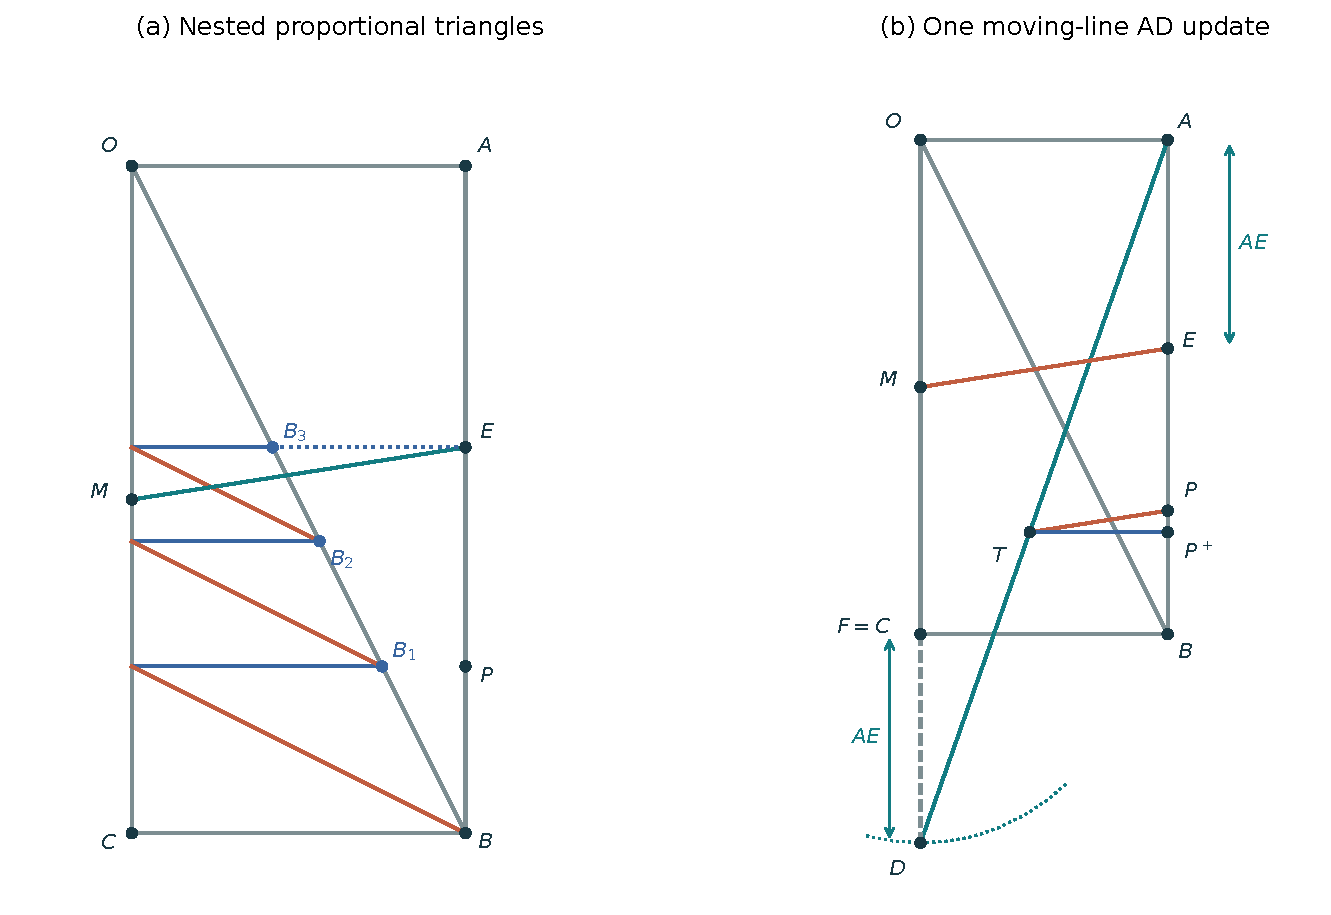
\includegraphics[width=.94\linewidth]{figures/geometry.pdf}
\caption{Geometric source of the update, retained from V17. For $p=3$, $X=W=2$, $H=4$, $s=3/4$, the proportional chain supplies $E$ and the moving support reports $P^+$. Extended lines are allowed. The fast circuit replaces the linear-length power chain by binary arithmetic; it does not physically reproduce this drawing.}
\end{figure}
The compass-based AD5 variants and projective constructions belong to the geometry companion. They are not implemented or electrically validated by the order-three circuit studied here.
\clearpage

\section{Preparation and bounded centered arithmetic}
\subsection{Digital preparation is part of the computation}
The controller accepts $p$ and a positive finite binary64 $X$. Certified interval comparisons and binary powering prepare a positive scale $c$ with $1\le Xc^p\le2$ and a rounded value $Y\approx Xc^p$. This uses the gallery's compact initializer and 128-bit interval arithmetic, not a root, logarithm or exponential oracle. Exact identities below use $Y=Xc^p$; rounding is an implementation error tested separately.

Write $s=cu$, initialize $u_0=1$, and store
\begin{equation}
 q=p(u-1),\qquad t=Yu^p,\qquad \widehat r=\frac{1}{c(1+q/p)}.\label{eq:state}
\end{equation}
For $p=10^6$, $X=500000$, preparation returns $c=0.9999871253967285$ and $Y\approx1.28104637891846$. Already $1/c$ has relative error about $2.477\times10^{-7}$. The analog computation refines a digitally prepared estimate: this initial accuracy cannot be credited to the analog core.

\subsection{Exact polynomial power stages}
Directly storing $u$ gives $\partial\log t/\partial u=p/u$. In contrast, $\partial\log t/\partial q=1/u$. For a partial exponent $n$, define $d_n=(p/n)(u^n-1)$, so $d_1=q$. Expansion gives
\begin{align}
 d_{2n}&=d_n+\frac{n}{2p}d_n^2,\label{eq:square}\\
 d_{n+1}&=d_n+\frac{q-d_n}{n+1}+\frac{n}{p(n+1)}d_nq.\label{eq:multiply}
\end{align}
The usual binary schedule evaluates $u^p=1+d_p$ with
$\lfloor\log_2p\rfloor+\operatorname{popcount}(p)-1$ stages: 25 at $p=10^6$ and at most 37 in the supported range. These are unrolled stages, not a demonstrated reuse of one physical multiplier.

\begin{proposition}[Ideal orbit bounds]
For exact preparation $1\le Y\le2$, the initialized positive AD orbit satisfies
\[
 Y^{-1/p}\le u\le1,\qquad -\log2<q\le0,\qquad q\le d_n\le0\quad(1\le n\le p).
\]
\end{proposition}
\begin{proof}
Positive Halley iteration in the inverse state preserves the interval from the root to the initial state; the V20 convergence results provide this invariance. If $Y>1$, $p(e^{-\log Y/p}-1)>-\log Y\ge-\log2$; $Y=1$ gives $q=0$. Finally $1-u^n=(1-u)\sum_{j=0}^{n-1}u^j\le n(1-u)$, which yields $d_n\ge q$; $u\le1$ gives $d_n\le0$.
\end{proof}
These real-arithmetic bounds motivate $\pm2$ V rails with one volt per unit state. They do not bound trajectories with offset, leakage or quantized coefficients. Simulation checks those trajectories explicitly.
\clearpage

\section{Centered correction and formal evidence}
Substituting \eqref{eq:state} into \eqref{eq:ad} yields
\begin{equation}
 \boxed{q^+=q+\frac{2(1+q/p)(1-t)}{1+t+(t-1)/p},\qquad t=Y(1+d_p).}\label{eq:centered}
\end{equation}
This is the same discrete AD map in new coordinates. In exact arithmetic the denominator is positive for $p>1$, $t>0$. The circuit's denominator floor is a numerical guard; activation invalidates a normal-operation claim.

A state error $\delta$ affects the decoded root through
\begin{equation}
 \frac{\widehat r(q+\delta)}{\widehat r(q)}-1
 =-\frac{\delta}{p+q+\delta},\label{eq:error}
\end{equation}
when the denominators are nonzero. This explains why large-degree root accuracy can remain good despite visible state errors. It also explains why testing only the million-degree example would be misleading. Low degrees are more demanding for the specified root-error target.

\textbf{Formalization map.} The module
\texttt{LeanMath.Papers.AnalogFastAD} contains the following six identities. They are compiled and audited separately from the earlier geometry library.
\begin{center}\small
\begin{tabularx}{\linewidth}{@{}lX@{}}\toprule
Lean declaration & Scope \\ \midrule
\texttt{centered\_square} & Expansion \eqref{eq:square}, with nonzero divisors.\\
\texttt{centered\_multiply} & Expansion \eqref{eq:multiply}, with nonzero divisors.\\
\texttt{centered\_ad} & Rational conjugacy \eqref{eq:centered}, with denominator hypotheses.\\
\texttt{scaled\_decode} & Algebraic identity $c(1+q/p)=c+cq/p$.\\
\texttt{normalized\_product} & $X(cu)^p=(Xc^p)u^p$.\\
\texttt{error\_scaling} & State-coordinate difference $\delta/p$.\\\bottomrule
\end{tabularx}\end{center}
The final two propositions should not be confused with a theorem about converter accuracy. In particular, \eqref{eq:error} is an elementary derivation in this article; the declaration \texttt{error\_scaling} certifies the affine state difference, not the full decoded relative-error formula.

The imported initialization library contains interval-acceptance, dyadic initialization and calibrated-orbit statements, including \texttt{positive\_dyadic\_initialization} and \texttt{orbit\_calibration}. Their hypotheses apply to exact real arithmetic. Compiling these statements does not constitute formal verification of the JavaScript implementation, SPICE solver, ADC, switch network, noise process or physical layout. The present six-identity module also does not newly formalize the ideal-orbit bound proved on the preceding page.

\textbf{What is preserved and what changes.} The ideal iteration retains its cubic local order. Finite electrical errors introduce bias and noise floors; an inexact physical iteration need not converge to the exact root. Replacing sampled iteration by continuous feedback changes the dynamics and does not inherit the discrete convergence theorem.
\clearpage

\section{Behavioral implementation and calibration}
\begin{figure}[H]\centering
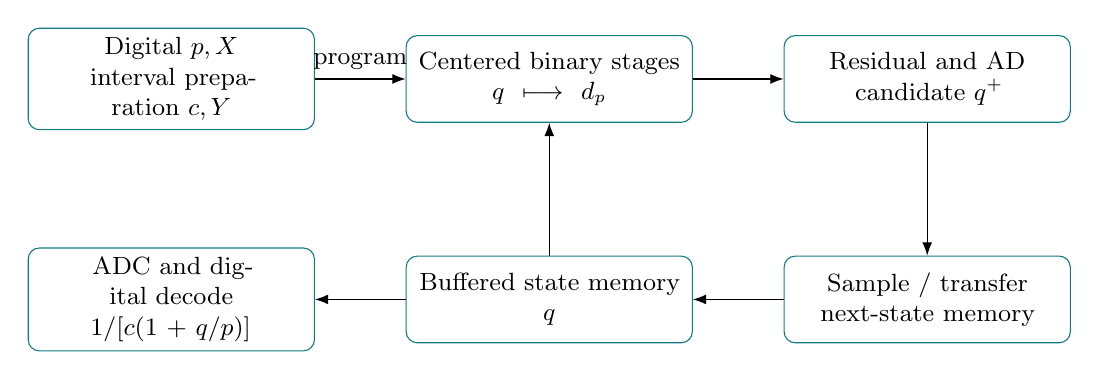
\begin{tikzpicture}[font=\small,>=Latex,box/.style={draw=teal,rounded corners,align=center,text width=3.4cm,minimum height=1.1cm}]
\node[box] (prep) at (0,2.8) {Digital $p,X$\\interval preparation $c,Y$};
\node[box] (power) at (4.8,2.8) {Centered binary stages\\$q\longmapsto d_p$};
\node[box] (ad) at (9.6,2.8) {Residual and AD\\candidate $q^+$};
\node[box] (state) at (4.8,0) {Buffered state memory\\$q$};
\node[box] (next) at (9.6,0) {Sample / transfer\\next-state memory};
\node[box] (out) at (0,0) {ADC and digital decode\\$1/[c(1+q/p)]$};
\draw[->] (prep)--node[above]{program}(power);
\draw[->] (power)--(ad);\draw[->] (ad)--(next);\draw[->] (next)--(state);
\draw[->] (state)--(power);\draw[->] (state)--(out);
\end{tikzpicture}
\caption{Functional architecture. Programming and conversion are not transistor-level implementations. Timing controls the sample and transfer switches; the noise-aware controller discussed later is a separate subsystem model.}
\end{figure}
The SPICE model uses behavioral polynomial and division sources, finite one-pole stage responses, input loading, buffered storage, switch resistance, leakage, charge injection and imposed disturbances. There are no manufacturer multiplier macromodels or foundry transistors. Noise is represented by seeded piecewise-linear voltage disturbances at 10~$\mu$s knots and sample disturbances, not by a comprehensive device-noise spectrum.

The precision revision begins with the earlier untrimmed error assumptions and adds physical mechanisms at the behavioral level:
\begin{center}\small
\begin{tabularx}{\linewidth}{@{}lXX@{}}\toprule
Parameter & Earlier combined model & Precision revision\\\midrule
Two hold capacitors & 10 nF each & 100 nF each\\
Switch on resistance & 120 $\Omega$ & 230 $\Omega$\\
Sample / transfer widths & 10 / 10 $\mu$s & 400 / 400 $\mu$s\\
Iteration period & 500 $\mu$s & 1,200 $\mu$s\\
Coefficient / ADC resolution & 16 / 18 bits & 24 / 24 bits\\
Readout & Last of six iterations & Mean of last 16 of 20\\\bottomrule
\end{tabularx}\end{center}
Four electrical-reference procedures calibrate the cells, memory drift, memory transfer and ADC. An 81-point DC grid fits arithmetic-cell corrections. Four memory reference voltages at two hold times estimate leakage; an assumed programmable current source compensates it with 2 pA resolution and $\pm1~\mu$A range. The transfer is then recalibrated. Seventeen ADC reference levels fit gain and offset; a sinusoidal one-LSB nonlinearity remains. Synthetic measurement uncertainty is 0.1~$\mu$V RMS.

No target root is used in calibration. Calibration is repeated at each tested temperature and schedule; drift after calibration is not covered. Reference accuracy, trim-source noise, capacitor tolerance, converter timing and trim-circuit area remain requirements, not demonstrated hardware. A 24-bit code does not imply 24 effective physical bits.
\clearpage

\section{Validation: broad coverage and precision revision}
The datasets answer different questions and must not be pooled as if every case exercised the final circuit. The broad arithmetic campaign evaluates 8,243 pairs, 4,278 distinct degrees and 24,729 arithmetic executions, with high-precision reference scoring. The largest recorded ideal relative error is approximately $1.14\times10^{-16}$. Inputs include extreme finite and subnormal binary64 values, random degrees and binary-boundary cases.

The earlier combined SPICE campaign comprises 148 pairs under each of two error profiles. Neither profile activates the range/denominator guards, but only 44/148 untrimmed and 97/148 tighter-profile results meet one ppm. Their worst errors are approximately 936 and 14.8 ppm. Numerical execution success is therefore not evidence of sufficient accuracy.

\textbf{Revised validation.} After development on three input pairs at two temperatures, the revised design is fixed. A separate set comprises 48 pairs from twelve degrees and four inputs, plus sixteen seeded random pairs. Temperature cycles through $-20,25,85\,^{\circ}$C; static-error signs and disturbance seeds vary. Paired original/revised execution produces 128 primary transients. All 64 revised results improve and meet one ppm: the largest error falls from 403.5 to 0.279 ppm \emph{on this set}. This is not the worst error from the earlier 148-pair campaign. A four-times-finer timestep check is performed on the worst revised case.
\begin{figure}[H]\centering
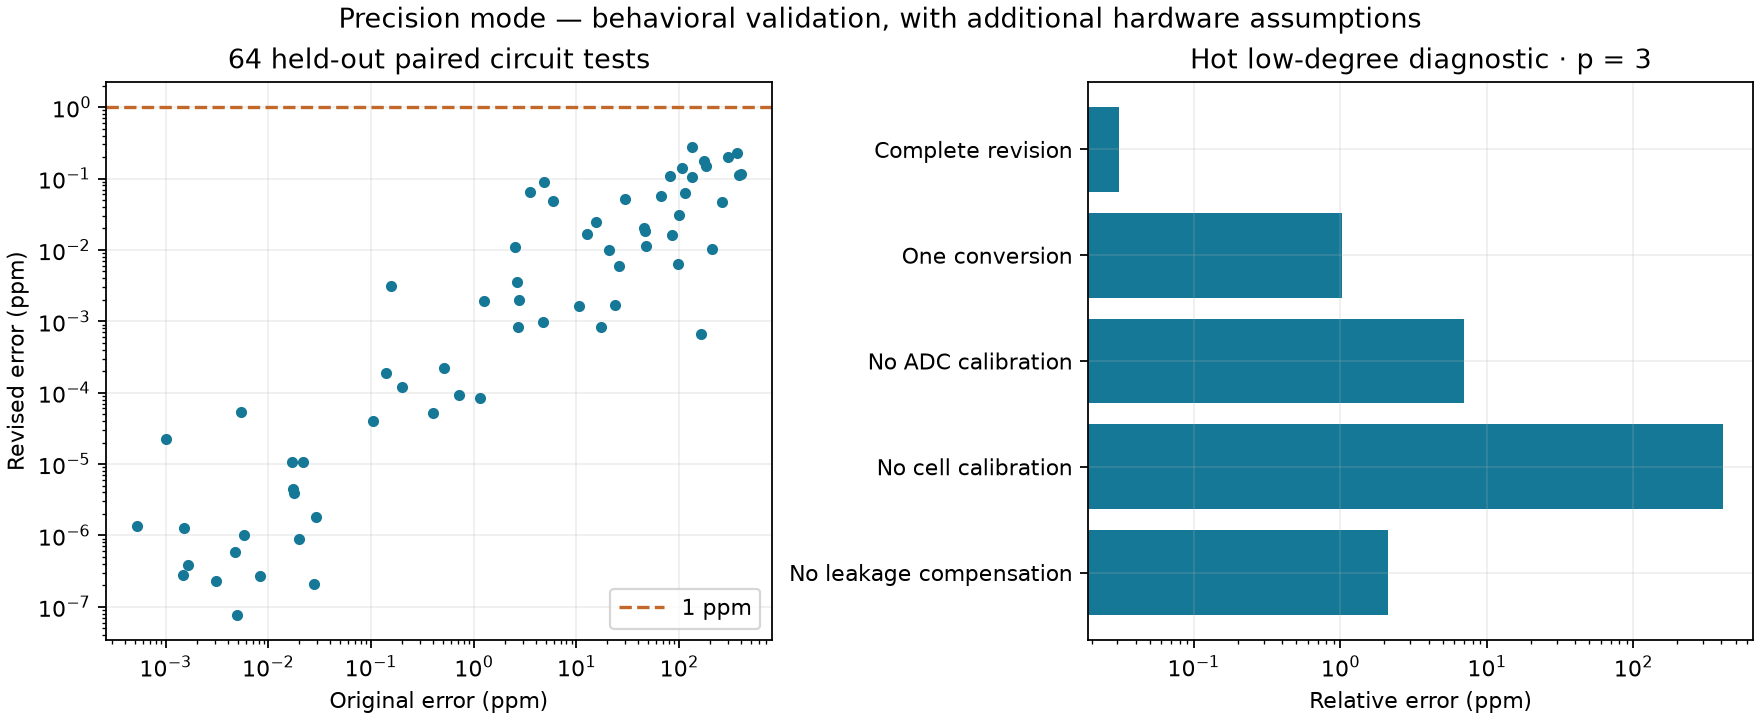
\includegraphics[width=\linewidth]{figures/precision_revision.png}
\caption{Left: paired precision-revision errors on 64 validation inputs. Right: one hot, low-degree diagnostic case, $p=3$, $X=0.037$, $85\,^{\circ}$C. The ablation results attribute improvements within that case; they are not universal per-block error bounds.}
\end{figure}
In the diagnostic case, removing cell calibration gives about 410 ppm, removing ADC calibration 6.94 ppm, and removing leakage compensation 2.10 ppm even after recalibrating the memory transfer. One final conversion gives 1.03 ppm; the complete averaged revision gives 0.031 ppm. Larger capacitors alone do not remove drift during arithmetic evaluation.

All accuracy figures use relative error in the decoded positive root, with high-precision scoring outside the simulated control loop. The 64 cases provide finite validation under specified assumptions, not a worst-case theorem, an exhaustive binary64 test or a manufacturing-yield estimate.
\clearpage

\section{Precision versus time}
The full precision schedule reads at 23.985 ms. A further study holds the component and error models fixed while varying five schedules and fixed readout policies. Forty development trajectories cover eight input pairs at $p=3,7,983039,10^6$. Policies use 2--20 iterations and 1--16 averaged states where allowed. Scoring prefixes of a trajectory does not create independent trials; stopping is fixed in advance, not chosen by consulting the true root.

The fastest development policy for each target is frozen before eighteen new input pairs are evaluated across six degrees, three input magnitudes, three temperatures and new seeds. Two distinct selected policies receive finer-timestep checks.
\begin{center}\small
\begin{tabular}{@{}rrrr@{}}\toprule
Target & Readout time & New cases passing & Largest error\\\midrule
100 ppm & 2.385 ms & 18/18 & 1.239 ppm\\
10 ppm & 2.385 ms & 18/18 & 1.239 ppm\\
1 ppm & 4.785 ms & 18/18 & 0.653 ppm\\\bottomrule
\end{tabular}\end{center}
The first policy reads the second iteration. The one-ppm policy averages iterations three and four. Retrospective evaluation on the earlier 64 precision trajectories also passes both targets, with maxima of 1.903 and 0.982 ppm respectively. This reused dataset is not a new independent campaign; the latter figure leaves little margin below one ppm.
\begin{figure}[H]\centering
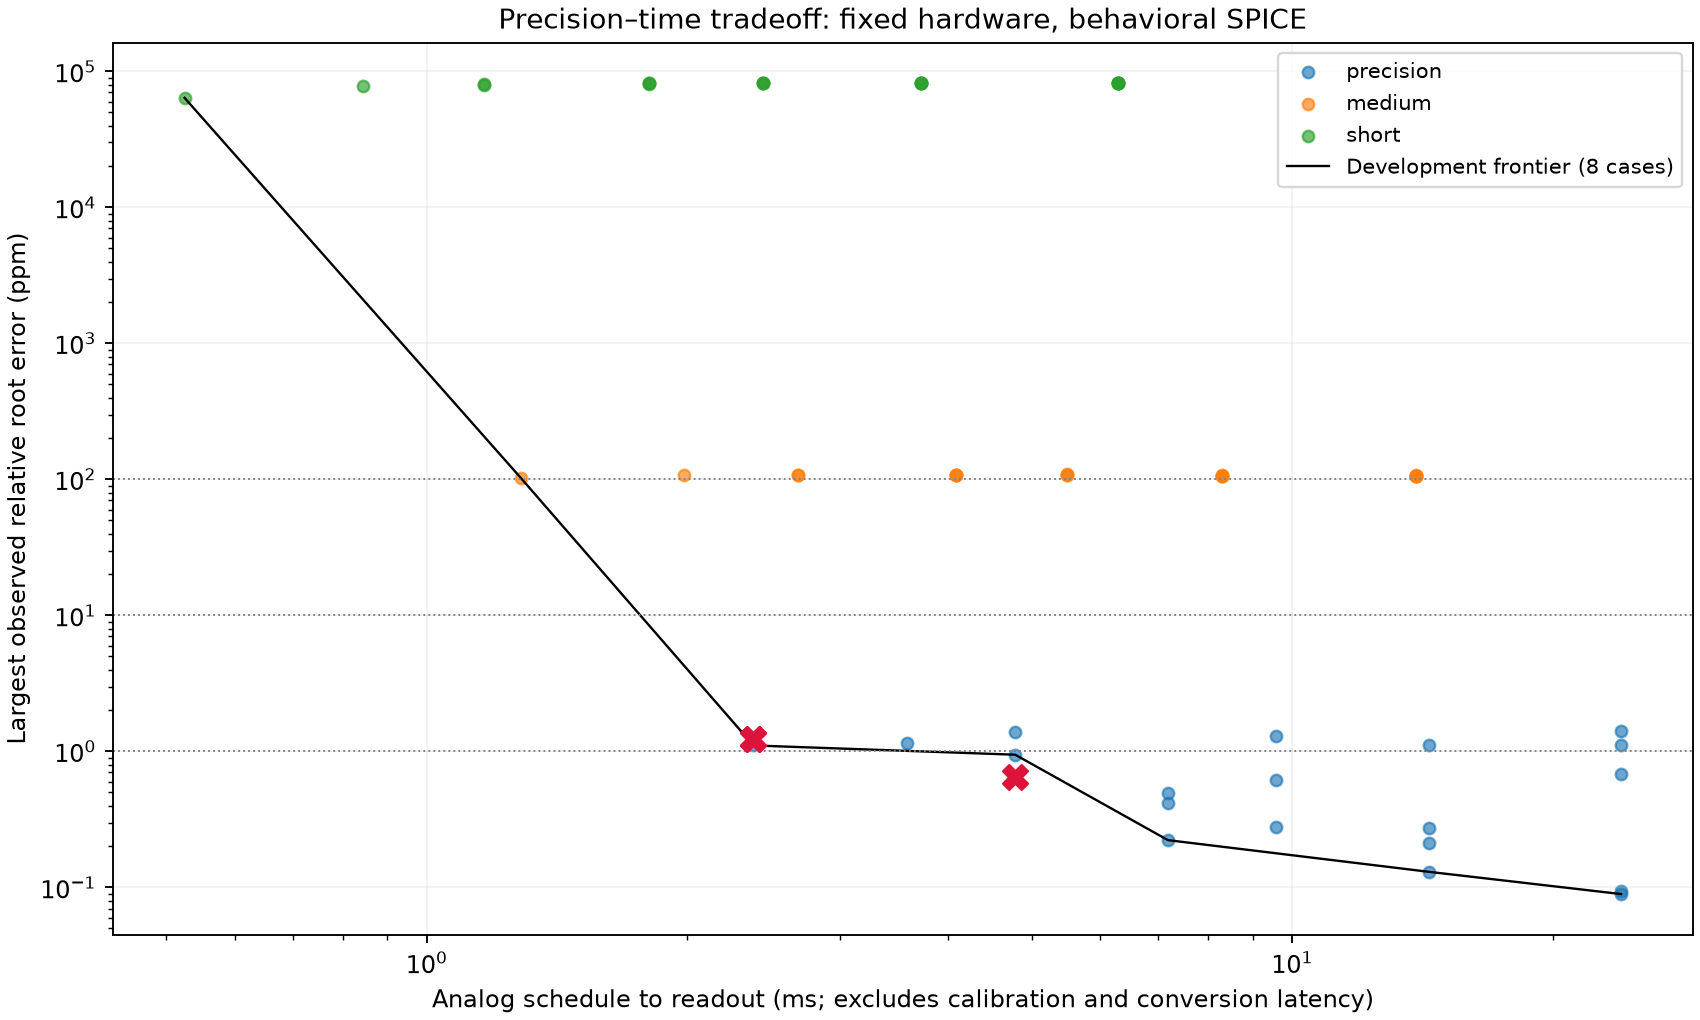
\includegraphics[width=.92\linewidth]{figures/speed_accuracy.png}
\caption{Largest observed error versus scheduled readout time. Colored points are fixed policies on the development set; red crosses are validation maxima. The connecting line is not an interpolated accuracy guarantee. Two more aggressive schedules have rejected trajectories and cannot enter the all-case frontier.}
\end{figure}
The reduction comes from fewer iterations and averaged readings. Narrowing acquisition windows with the same hardware produces large low-degree errors and, for aggressive settings, out-of-range signals. It does not demonstrate a faster accurate device.
\clearpage

\section{Timing interpretation and alternatives to a clock}
The quoted milliseconds are modeled elapsed time from a prepared job and prescribed state reset to its required readout. They are neither simulator wall-clock time nor supply startup time. They exclude interval preparation, coefficient programming, electrical calibration, physical ADC conversion latency and final digital decoding. Thus they are not measured end-to-end chip latency.

An already powered analog circuit still has to change stored voltages when its input changes. Preserving the previous state can help nearby inputs but is not equivalent to having the new answer preloaded. The timing study resets the prescribed state and does not measure continuous tracking. An earlier 196-job streaming experiment retains arithmetic-stage states while resetting $q$ and ideally reprogramming coefficients; it excludes the revised circuit errors and converter delays.

\textbf{Event-driven sampled updates.} A separate noisy completion-controller model includes detector offset, 2~$\mu$V RMS disturbances, 20-bit detector quantization over 4 V, 12/24~$\mu$V hysteresis, 10~$\mu$s dwell, a delay-bound guard and timeout. Eighteen normal jobs complete. Four injected stuck-candidate or excess-noise cases time out without transfer. Step refinement is also checked. The model assumes a characterized upper stage-delay bound and ideal memory transfer. It is not connected to the revised SPICE memory and ADC; it does not yet establish a physical clockless implementation.

\textbf{Continuous feedback.} Fifty-two earlier feedback transients include timestep refinements and extended observations. Fast feedback can oscillate or hit guards. At an intermediate setting, the million-degree case settles during the extended observation while the 37-stage case still oscillates. Continuous feedback therefore requires its own stability study; the discrete Halley theorem does not settle this question.

\section{Position relative to existing computation}
The host benchmark uses warmed-up JavaScript, varying inputs and batches on an Apple M5. For $p=10^6$, $X=500000$, recorded median per-call times are approximately 13 ns for \texttt{exp(log(X)/p)}, 0.69~$\mu$s for six already-prepared digital AD steps, and 179~$\mu$s for preparation plus digital AD. These are amortized host-loop timings, not universal isolated latencies. Nonetheless the present evidence establishes no analog speed advantage. Energy and silicon area have not been measured.

Analog roots are not a new capability. The commercial AD538 supports resistor-programmed powers with exponent 0.2--5; its documented range does not directly implement $p=10^6$ \cite{ad538}. Tatulian and DeMara describe a reconfigurable spin-based analog block explicitly targeting generalizable $n$th powers and roots \cite{spin}. These are relevant antecedents, not equivalent benchmarks: input representation, precision, degree programming and validation maturity differ. We make no priority or best-in-class claim. A common accuracy and input-range specification, including preparation and conversion, is required for a meaningful hardware comparison.
\clearpage

\section{Reproducibility and conclusions}
The implementation snapshot underlying this article is commit \texttt{e954910} of \repo; the paper and its build instructions are added subsequently. The archive preserves the exact scripts and recorded results, including rejected settings. Build instructions are in \texttt{paper/pandrosion\_analog\_v30/README.md}.

\begin{center}\small
\begin{tabularx}{\linewidth}{@{}lX@{}}\toprule
Repository location & Evidence\\\midrule
\texttt{LeanMath/Papers/AnalogFastAD.lean} & Six exact identities.\\
\texttt{scripts/audit\_analog\_fast\_ad.py} & Separate proof audit.\\
\texttt{research/analog\_fast\_ad/} & Scripts and raw numerical records below.\\
\quad\texttt{generalist\_campaign.py} & Broad arithmetic coverage.\\
\quad\texttt{generalist\_spice.py} & Earlier paired timed error profiles.\\
\quad\texttt{validate\_revised.py} & 64-pair precision validation.\\
\quad\texttt{revised\_ablation.py} & Five diagnostic runs.\\
\quad\texttt{speed\_accuracy.py} & Timing selection and new validation.\\
\quad\texttt{noisy\_controller.py} & Separate completion and fault tests.\\\bottomrule
\end{tabularx}\end{center}
Independent SPICE reruns require ngspice, Node.js for the actual initializer, and the listed Python dependencies. Random seeds and fitted calibration values are retained. CI rebuilds the mathematics and papers and reruns the circuit campaigns. A successful CI run certifies execution of those checks, not physical-device quality. The paper's compact result checks compare its numerical summary with the retained JSON records.

\textbf{Remaining engineering work.} The main unresolved steps are transistor- or component-level implementation of arithmetic and trims; realistic converter and reference models; capacitor tolerance and correlated drift; integration of completion detection with noisy storage; input reconfiguration; and power, area and layout extraction. The 2 pA current trim and 0.1~$\mu$V calibration uncertainty must be realized, not merely specified. These are a further hardware-design phase.

\textbf{Conclusion.} Centering the state and every partial power provides an exact arithmetic route from the AD geometry to a bounded-signal, high-degree mixed-signal prototype. The broad campaigns show why high degree alone is not a sufficient precision test. Electrical calibration and longer acquisition improve low-degree behavior in the stated model; early readout then trades precision margin for time. The strongest present claim is reproducible, finite-case behavioral feasibility supported by exact algebraic certificates. It is not a fabricated root-calculator specification or a demonstrated improvement over optimized digital computation.

\begin{thebibliography}{9}\small
\bibitem{repo} I. Besevic. \emph{Pandrosion research repository}. Source, data, Lean proofs and interactive gallery. \repo.
\bibitem{v20} I. Besevic. \emph{Reciprocal Root Geometry}, V20, and \emph{From Proportional Rectangles to Sampled Analog Root Computation}, V17. Archival companion manuscripts in the repository.
\bibitem{ad538} Analog Devices. \emph{AD538: Real-Time Analog Computational Unit}, Rev. E. \url{https://www.analog.com/media/en/technical-documentation/data-sheets/ad538.pdf}.
\bibitem{spin} A. Tatulian and R. F. DeMara. \emph{A Reconfigurable and Compact Spin-Based Analog Block for Generalizable nth Power and Root Computation}. IEEE ISVLSI, 2021. DOI: \href{https://doi.org/10.1109/ISVLSI51109.2021.00062}{10.1109/ISVLSI51109.2021.00062}.
\end{thebibliography}
\end{document}
